% Title:    A LaTeX Template For Responses To a Referees' Reports
% Author:   Petr Zemek <s3rvac@gmail.com>
% Homepage: https://blog.petrzemek.net/2016/07/17/latex-template-for-responses-to-referees-reports/
% License:  CC BY 4.0 (https://creativecommons.org/licenses/by/4.0/)
\documentclass[11pt]{article}

\usepackage{amsmath,amssymb}
\marginparwidth 0pt
\oddsidemargin  0pt
\evensidemargin  0pt
\marginparsep 0pt
\topmargin   -0.25in 
\textwidth   6.5in
\textheight  9.0in
% Allow Unicode input (alternatively, you can use XeLaTeX or LuaLaTeX)
\usepackage[utf8]{inputenc}
\usepackage{color,nima}
\newcommand{\outNim}[1]{}

\usepackage{hyperref}

\usepackage{microtype,xparse,tcolorbox}
\newenvironment{reviewer-comment }{}{}
\tcbuselibrary{skins}
\tcbuselibrary{breakable}
\tcolorboxenvironment{reviewer-comment }{empty,
  left = 1em, top = 1ex, bottom = 1ex,
  borderline west = {2pt} {0pt} {black!20},breakable
}
\ExplSyntaxOn
\NewDocumentEnvironment {response} { +m O{black!20} } {
  \IfValueT {#1} {
    \begin{reviewer-comment~}
      \setlength\parindent{2em}
      \noindent
      \ttfamily #1
    \end{reviewer-comment~}
  }
  \par\noindent\ignorespaces
} { \bigskip\par }

% \NewDocumentEnvironment {response} { +m O{black!20} } {
%   \IfValueT {#1} {
%     \begin{tcolorbox}[breakable]
%         \setlength\parindent{2em}
%       \noindent
%       \ttfamily #1
%     \end{tcolorbox}
  
%     % \begin{reviewer-comment~}
%     %   \setlength\parindent{2em}
%     %   \noindent
%     %   \ttfamily #1
%     % \end{reviewer-comment~}
%   }
%   \par\noindent\ignorespaces
% } { \bigskip\par }


\NewDocumentCommand \Reviewer { m } {
  \section*{Comments~by~Reviewer~#1}
}
\ExplSyntaxOff
%\AtBeginDocument{\maketitle\thispagestyle{empty}\noindent}

% You can get probably get rid of these definitions:
\newcommand\meta[1]{$\langle\hbox{#1}\rangle$}
\newcommand\PaperTitle[1]{``\textit{#1}''}

\title{Statement on the Revision of \meta{Paper ID} \\
  Based on the Referees' Report}
\author{Author1 \and Author2 \and Author3}
\date{\today}
\usepackage{setspace}
% \onehalfspacing
 \linespread{1.5}

\begin{document}


% This statement concerns our revision of the \meta{Paper ID} paper,
% entitled \PaperTitle{\meta{Paper Title}}, based on the referees' report.
\outNim{
\subsection*{TODO}

 \linespread{1}

\begin{enumerate}
    \item Code online
    \item Why using $d\log\be{R}/d\log r_N$? 
    Advantage over $dV/dr$?
    \item Wouldn't it be a first order transition if slope of $V $ shows discontinuity?
    % \item Complexity details
    % \item Phase graph for 3D random geometric graphs.   
    % \item Transition point not scaling with size. Discuss correct choice of $N,L$. 
    % \item curvature  
    % \item Discuss why relaxation time of ELI is not peaked
    % \item Calculate finite size scaling of transition region. 
\end{enumerate}
}%%%%
 \linespread{1.5}
\Reviewer{\#1}

\begin{response}{
Characterizing the network geometry of networks is a topics of significant scientific interest and it is fundamental for understanding the architecture principles of the connectome and for the designing 3D integrated circuits. This manuscript provides a theoretical framework and an algorithm applicable to any network topology to characterize the network geometry in 3D when links have a give thickness and link crossing are forbidden.
While the optimization problem addressed by this manuscript is NP hard, the proposed algorithms are able to find the energetically favourable local minima and avoid link crossing. The conducted investigation over a large variety of networks reveals an universal phase transition between a weakly interacting phase and a strongly interacting phase as a function of the links thickness. The network physical properties are tested by applying external forces and monitoring the network response. It is found that the observed phase transition corresponds to a solid and fluid gel-like response to stress.
The work is highly innovative and very important to reveal the network geometry underlying complex networks. As such it has a wide realm of applications and it will be important for a large variety of disciplines. I believe that this work together with the rich Supplementary Material are suitable for publication in Nature.
However I would like to raise few comments that the Authors might consider to address for their resubmitted revealing the wide range of questions that such work can generate.
}
We thank the referee for the excellent summary of the paper's results and the gracious comments on its potential impacts on the community. 

\end{response}

\begin{response}{
1) First of all I believe that a freely available codes would be very important for busting the research in this field. Are the Authors thinking of publishing their code?
}
We fully agree. 
We are , therefore, sharing 
all of the simulation source code in Python, together with an example code in Jupyter notebook, on Github. 
The link is \texttt{\href{https://github.com/nimadehmamy/3D-ELI-FUEL}{github.com/nimadehmamy/3D-ELI-FUEL}} where we plan to update and perfect the code. 
We are also adding to it a web-based tool to visualize and interact with the simulations in 3D (\texttt{\href{http://nimadehmamy.com/3dviz}{nimadehmamy.com/3dviz}}).

%{\color{red} Include URL?} 
\end{response}
\begin{response}{
2) An analysis of the computational complexity of the algorithm would be relevant, how does the time of computation and the memory needed to store these physical networks scale with the network parameters?
}
This is, indeed, a key point. 
Therefore Sec. SI 8.C now offers a detailed analysis of the time complexity of the algorithm. 
Briefly, if each link had $s$ segments, each iteration has the following time complexities:
\begin{enumerate}
    \item {\bf Brute-force:}  elastic forces is $O(sL)$;  node repulsion is $O(N^2)$; and link repulsion $O(s^2L^2)$. 
    Since for a connected network $L\geq N-1$ and $s>1$, the total complexity is usually $O(s^2L^2)$.  
    \item {\bf Exploiting short range of link repulsion:}
    We only need short-range link repulsion to avoid crossings. 
    Partitioning the space into cubic cells of size $ar_L$ (with $a \sim O(1)$; we chose $a=4$) we will capture most of the link repulsions by considering interactions within cells.
    With cells the worst case complexity becomes $O\pr{s^2a^3 L^{3/2}}$ (SI 8.C).
    % \item {\bf Update cells:} We update the cells and change their location randomly every few (50-100) iterations to better capture all interactions. 
    % Updating cells is $O(sL)$.
    \item {\bf Reduced complexity:} 
    A modified version, only calculating link repulsion for $c$ link pairs instead of all pairs in a cell, has complexity 
    $O\pr{c L^{3/2}/ a^3}$ (SI 8.C)
\end{enumerate}
In the strong phase, the reduced complexity $O\pr{c L^{3/2}/ a^3}$ after partitioning can be considerably better than the brute-force  $O\pr{s^2 L^{2}}$.
% Thus if we partition the space into cubic cells where the sides have length a few times $r_L$ we will capture most of the significant link repulsions by only considering interactions within these cells.
% We only need to compute the repulsive forces for pairs of link segments that are inside the same cell, as these are the only ones with a considerable repulsive force. 
% We update the cells and change their location randomly every few iterations to better capture all potential link interactions.
% With cells of size $ar_L$ and links with $s$ segments the worst case complexity of each iteration becomes $O\pr{s^2a^3 L^{3/2}}$ (SI 8.C).
% A modified version which only calculates the link repulsion for $c$ link pairs instead of all link pairs within a cell has complexity 
% $O\pr{c L^{3/2}/ a^3}$ (SI 8.C), which can be considerably better than the brute-force  $O\pr{s^2 L^{2}}$.
As in the weak phase link crossings are rare, most cells will contain a single link.
Thus, in the weak phase partitioning the space reduces the complexity of link repulsion so much that it may become less than the brute-force complexity of node repulsion, $O(N^2)$.
Therefore,  with partitioning the time complexity in the weak phase will be $\max\{O(N^2),O(sL)\}$, where $O(sL)$ is the complexity of partitioning the space (same as the elastic forces).


Discussion of the computational complexity is crucial for assessing the feasibility of any algorithm and we thank the referee for bringing this up. 
We will definitely extend SI 8.C to include the above.
This discussion is also useful for understanding the structure of  simulation code and the choices made therein.
The simulation code may achieve an even better time complexity by making use of a Binary Space Partitioning, such as a k-d tree, replacing the uniform cells that we have currently implemented.


\end{response}
\begin{response}{
3) Random geometric graphs are actually geometrical networks including a lot of link crossings. I imagine that one could observe a difference between the phase transition between the weak-interacting phase and the strong interacting phase for random geometric graphs in 2D or in 3D. My intuition is that for 3D random geometric graphs well deep in the percolation phase maybe the weak interacting phase disappear or else is significantly reduced. However for random geometric networks in 2D it is more easy to use the third dimension of the physical embedding to avoid crossings. 
}

This is an interesting scenario. 
Note that a random geometric graph (RGG) in 3D shares some characteristics of a force-directed layout (FDL) of an Erd\"os-Renyi (ER) random graph: 
1) in both networks nodes have a peaked degree distribution, thus nodes have similar degrees and have similar density of links around them; 2) in FDL nodes that are connected are on average closer to each other than disconnected nodes, similar to an RGG (One can argue that any ER graph is a RGG in $N-1$ dimensional space). 
Since our analysis shows that (Eq.(4)) the density of links is the important factor in the phase transition, we expect 3D RGG to behave similar to ER. 
For a 2D RGG, if the referee is asking about a 2D RGG with nodes fixed in a 2D plane inside 3D space, we do believe that phase transition will be slightly altered. 
The assumption of Eq.(4) is that nodes and links are distributed either randomly in space or based on FDL, which utilizes all three dimensions. 
Restricting the nodes to 2D would result in many link crossings even at very small $r_L$. 
As a result, the weak phase may disappear entirely. 
{\color{red}\bf  Find full phase space of 2D and 3D RGG}

The referee is pointing out an important aspect of our model. 
When the symmetries of 3D space are restricted, for instance by restricting nodes to a 2D subspace, the transition point may be affected. We are adding an explanation in the text, clarifying the underlying assumptions for Eq.(4) to be valid.
% Another aspect of these assumptions

% There are multiple, interesting scenarios that may pertain to the referee's question. 
% If the referee is assuming we start from a 2D random geometric graph (RGG), laid out on a plane, and then use our ELI algorithm in 3D to resolve its crossings while keeping nodes fixed, then, yes. 
% There would not exist any weakly interacting phase, as a large number of links have conflicts from the beginning. 
% {\color{red} TEST!!! This would arise from the  unusual symmetry of this setting}
% Note that in 2D any non-planar graph will have unresolvable link crossings. 
% This will include random geometric graphs. 
% So, in this sense, the referee's intuition is correct and the weakly interacting phase essentially disappears deep in the percolation phase. 
% %But, maybe the referee's question is about embedding a 2D random geometric graph in 3D, or ? 
% However, if you are asking whether for a 3D random geometric graph the weakly interacting phase disappears, we would argue that it does not. 
% %{\color{red} ER $\sim$ geometric, but not in 3D necessarily! show plots and sims!}

% Note that any force-directed layout (FDL) puts connected nodes closer to each other than non-connected nodes, which is also the formation criterion for a random geometric graph. 
% Thus, any FDL is equivalent to a random geometric graph which starts from a non-uniform spatial distribution of nodes.
% On the other hand, Erd\"os-Renyi (ER) random graphs have peaked degree distribution similar to random geometric graphs and FDL results in fairly uniform distribution of nodes in space (One could argue that any ER graph is a random geometric graph, just in a high dimensional space).  
% Based on this, 3D random geometric graphs must behave similar to random graphs. 

\end{response}

\newpage

\Reviewer{\#2}
\begin{response}{The authors examine the implications of spatial constraints (non crossing conditions of links and nodes) on the topology of networks embedded in a 3-dimensional space. 
Their main finding is that, depending on the link thickness ($r_L$), there exists two different phases with different geometrical properties, separated by a second order phase transition point occurring at a critical value $r_c$, which is approximated analytically. 
Physical properties of the network are shown to be substantially different in the two phases, and universality is claimed at the critical point. 
}

We thank the referee for the succinct summary of our main findings. 
\end{response}


\noindent
Main points:
\begin{response}{
1) The main analytical result of this work is the estimation of the critical radius in Eq.(4). 
The simple argument given in the main text is not satisfactory. 
The argument given by the authors disregards completely the heterogeneity in the density profiles of nodes and links, which are instead assumed to be uniform over the space. 
For example, in a scale free network, the density of links will be much higher near a hub node than low degree nodes, and these fluctuations may be strong enough to invalidate the argument used to derive Eq.(4), which assumes the same density around every node for example, in a scale free network with degree exponent $\gamma=2$, all links are basically 
attached to a single node (i.e. the node with largest degree), while in a 3D lattice they are evenly distributed across all nodes. Therefore, I do not see how the critical value $r_c$ cannot be sensitive to the value of the degree exponent $\gamma$, and thus on the network topology. Since the authors claim a "deep" universality, their main analytical finding Eq.(4) does not follow from this claim.

}

The referee brings up a key point: how does the degree heterogeneity affect the layout and the resulting phase transition? 
Indeed, as the referee correctly notes near a hub we often need to fit orders of magnitude more links than near a small degree node. 
%This is one of the reasons we have scaled the node sizes in the visualizations (see SI 7). 
Following the referee's suggestion, we have done a more careful evaluation of the transition point, which includes the effect of degree heterogeneity. 
The new derivation yields a degree-dependent condition for the transition around a node of degree $k$ as  

\begin{align}
    % \rho_+(k) 
    % &=\frac{A^{\frac{2}{3}} + 12 a}{6 \sqrt[3]{- A}}, &
    % A& = 12 \pr{9 b + \sqrt{(9b)^{2}- 12 a^{3} }}\cr
    \tilde{r}_c(k) = {r^c_L\over r_N} 
    &=\frac{6A^{{1\over 3}}}{A^{\frac{2}{3}} + 12 a}, &A& =- 12 \pr{{ 3k^{3/2}\over \alpha } + \sqrt{{ 9 k^{3}\over \alpha^2 }- 12 a^3 }},\quad a = {c\over \alpha}{L\over N^{2/3}} \label{eq:trans-rc-full-1}
\end{align}
where $\alpha = 4\sqrt{2}/\pi $ comes from close-packing of spheres in 3D and $c = O(1)$ depends on the distribution of linked nodes. 
For $\gamma = 2$, Erd\"os-Renyi (ER) and a star-shaped network $c = 3/4$. 
From \eqref{eq:trans-rc-full-1} we are able to find the transition point by averaging over the degree distribution. 
Furthermore, \eqref{eq:trans-rc-full-1} can be used to estimate finite-size effects due to degree heterogeneity by finding the standard deviation of $\tilde{r}_c(k)$ over the degree distribution. 
By doing so, we are able to identify the finite region in phase space where the phase transition is occurring. 
We have updated the phase-diagram accordingly. 

\begin{figure}
    \centering
    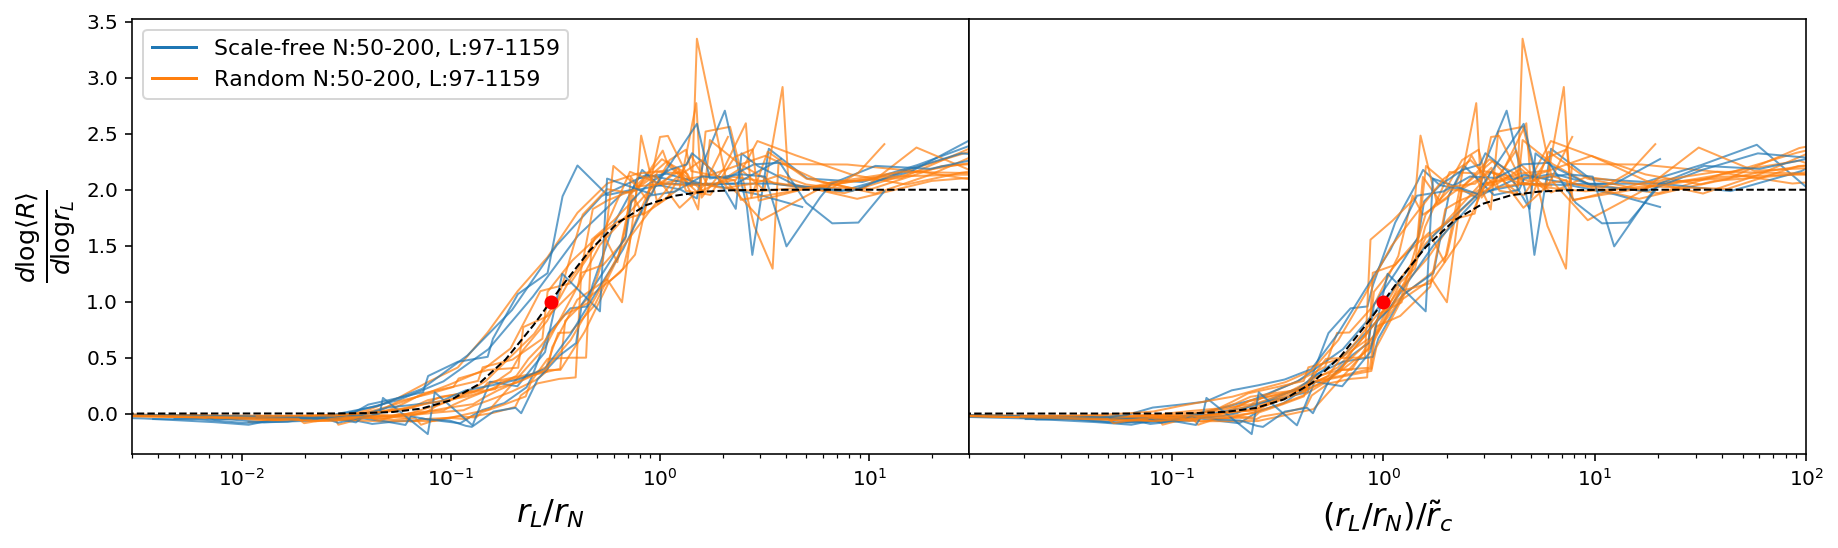
\includegraphics[width=\textwidth]{fig-09-19/phase-collapse-040918.png}
    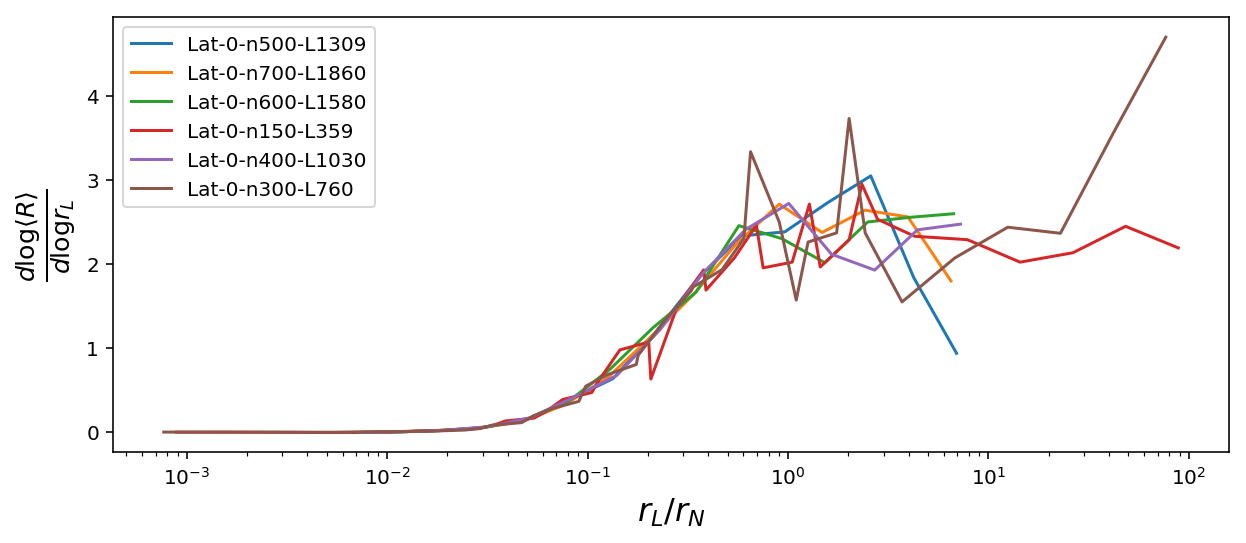
\includegraphics[width=.6\textwidth]{fig-09-19/phase-lat-040918.png}
    \caption{{\bf Phase transition vs Topology:} The quantity $\phi(r_L)\equiv d\log\be{R} /d\log r_L$ distinguishes well between the two phases  ($\be{R}$ being the average link length and keeping $r_N$ constant.)
    $\phi (r_L) $ is zero deep in the weak phase and it approaches $1$ deep in the strongly interacting phase. 
    While scale-free or random networks of various sizes network result in transitions occurring at different values of $r_L/r_N$ (Top, left), scaling by the predicted transition point $\tilde{r_c}=r^c_L/r_N$ collapses the curves well onto a single curve (Top, right).
    Lattice (Bottom) behave differently than random and scale-freee networks. 
    Lattice of all sizes have the same transition point, because once the unit cell has a phase transition the whole lattice udergoes a transition. 
    % If we start from the perfect lattice layout, the layout remains a lattice only gets slightly distorted at large $r_L$. 
    % The transition behavior in lattices is almost independent of the lattice size. 
    % 
    }
    \label{fig:phase-collapse}
\end{figure}

{\color{red} Table or plot of transition points and width for BA and ER. }

We also show that in the thermodynamic limit where $N\to \infty$ \eqref{eq:trans-rc-full-1} reduces to our previous approximation $\tilde{r}_c = \sqrt{{\alpha \over c}} N^{1/3}L^{-1/2}$. 
Note that $\sqrt{\alpha/c} \approx 0.9$ for ER and star-shaped networks. 
The derivation of this result assumes that links are distributed at all distances from the node. 
This assumption that holds for random networks as well as scale-free networks (as most nodes are connected to hubs and thus links connecting to hubs may extend from any part of the layout to the hub). However, it fails for lattices and random geometric graphs (RGG). 
In general, networks that are composed of identical (such as a unit cell in the lattice), or nearly identical sub-graphs (as in RGG) connected to each other over a metric space will rarely have very long links and the average length of a links will be independent of network size. 
Thus in lattices and RGG, the transition point and the spread of the transition region will be independent of network size. 
{\color{red} show Figure}

In conclusion, the referee raised a very important point about the effect of degree heterogeneity, which led us to a much more rigorous and precise derivation of the phase transition and some caveats about it. 
Additionally we augmented our derivation with finite-size scaling analysis, which we discuss further below.

\end{response}
\begin{response}{
2) Is the model in Eq.(1) a new model or has been already used in the literature? In the latter case, please provide a reference for the model Eq.(1). 
}
It is a new model, though similar models have been used in self-avoiding polymer chains \cite{des1974lagrangian} and manifold dynamics \cite{mezard1991replica}. 
Without $V_{LL}$ and replacing $V_{el}$ with the elastic energy of a spring yields the potential for a Force-directed layout with short-range node repulsion.  
\end{response}
\begin{response}{
3) What does it mean "the lowest energy solution of (1)"? Equation (1) is just the definition of the potential energy. Perhaps the authors meant the solution to the equation grad V = 0. Is that right?
}
We do mean lowest energy state of the potential, which corresponds to the ideal layout, though we also use $\del V=0$ as we will explain here. 
Similar to FDL, the premise is that we want to minimize distance of nodes that are connected to each other while avoiding node and link crossing. 
Long links have a large elastic energy $V_{el}$, and crossing nodes and links have high values of $V_{NN}$ and $V_{LL}$ respectively. 
Thus, the configuration with minimum $V$ is the most desirable one. 
The procedure we use to find the minimum is gradient descent with noise (simulated annealing, Eqs.(2,3)), which does find a local minimum which satisfies $\del V = 0$. 
But it also escape local minima with high $V$ due to the noise. 
\end{response}
\begin{response}{
4) The data collapse in Fig.1G looks quite poor, and the use of a log scale on the y-axis is misleading? I do not think this result can be taken as a confirmation of the scaling relation Eq. (4). 
}
\begin{figure}[ht]
    \centering
    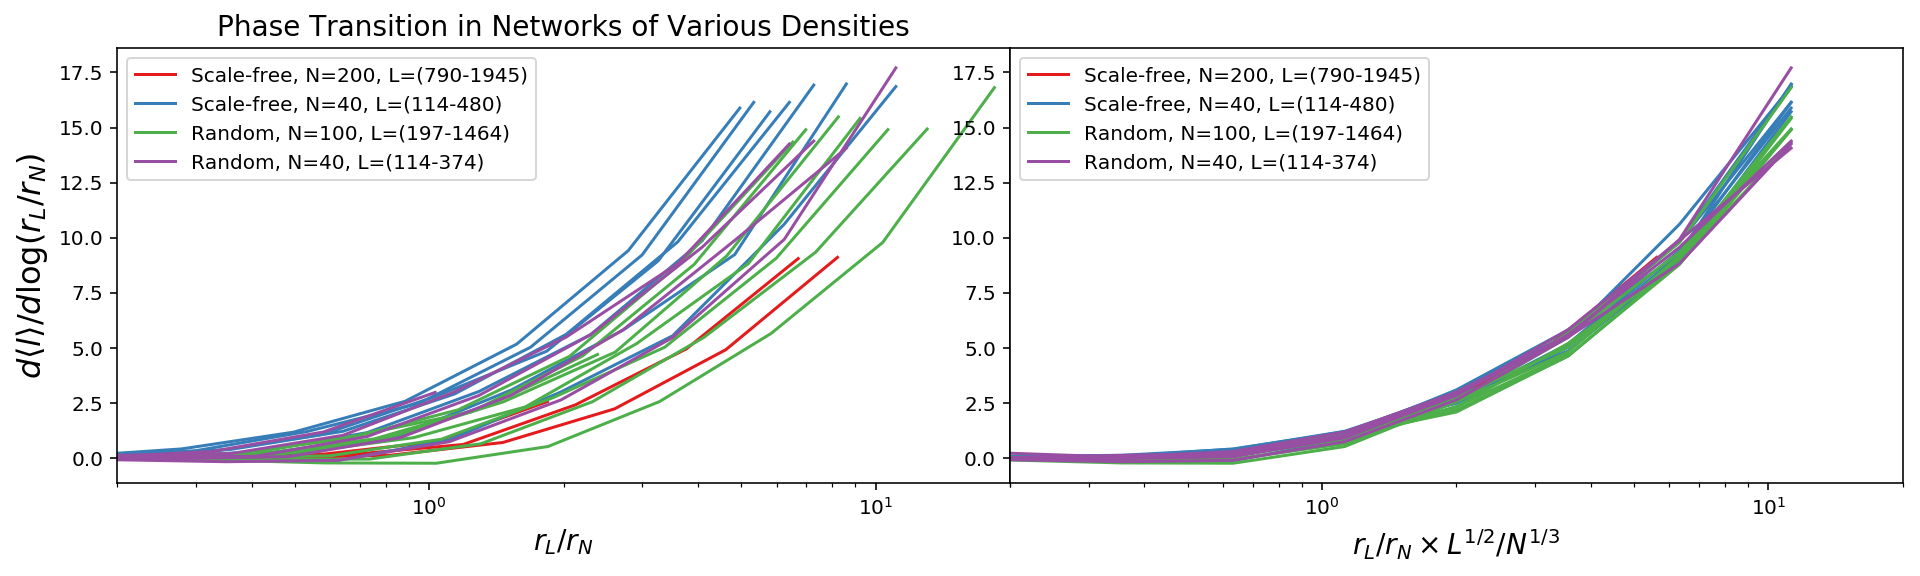
\includegraphics[width=\textwidth]{fig-09-19/trans-collapse-dlog.png}
    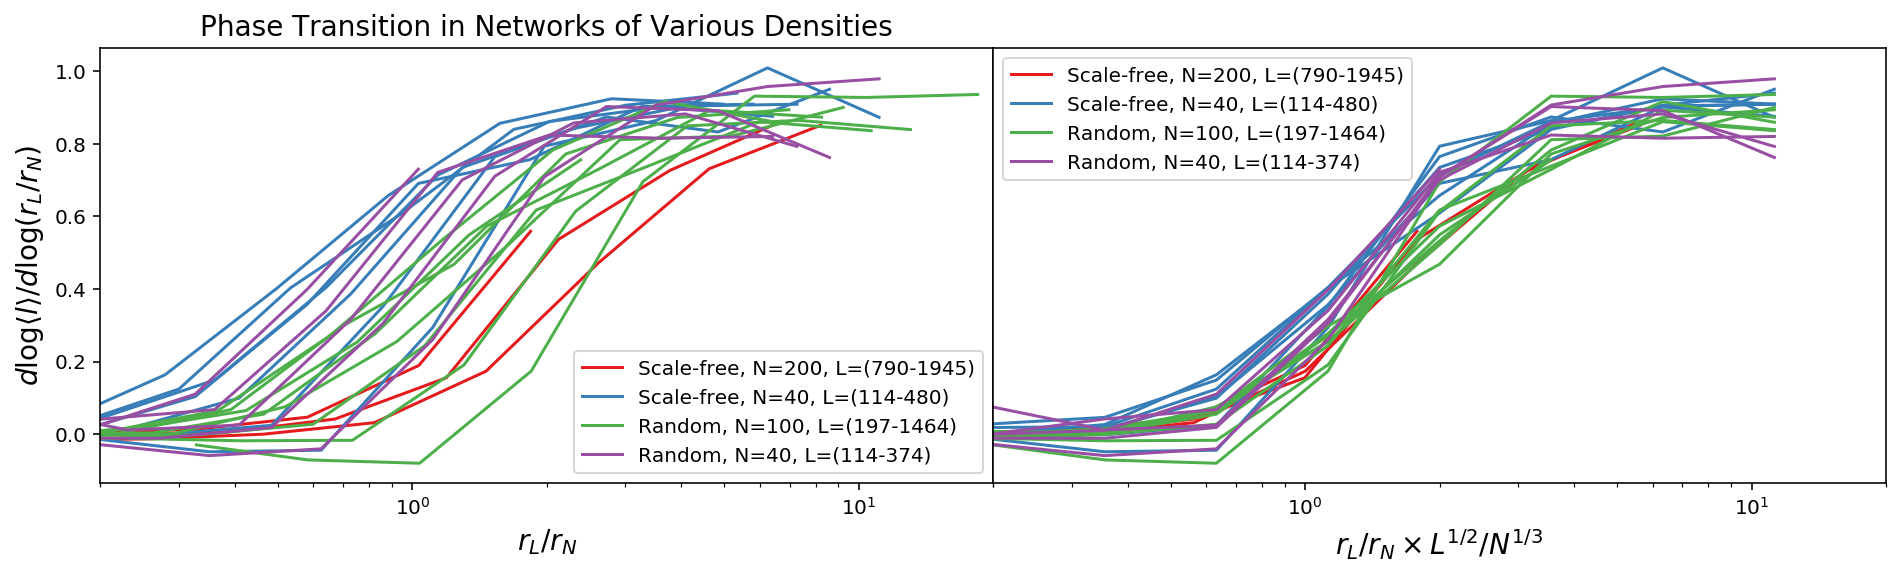
\includegraphics[width=\textwidth]{fig-09-19/trans-collapse-dlog2.png}
    \caption{{\bf The slope of the average link length:} Top shows the derivative of average link length $\be{l}$ with respect to $\log(r_L/r_N)$. 
    As we see, without rescaling (top left) the curves for different network sizes and topologies follow different trajectories. 
    After rescaling by the predicted scaling of the transition point (top right), all the curves collapse to a single curve. 
    Note the y-axis is in linear scale. 
    Also, note that the slope is zero and starts becoming nonzero after the transition point. 
    The bottom plots show the slope of the logarithms $d \log \be{l}/d \log (r_L/r_N)$. 
    Again, before rescaling (bottom left) they differ, but after rescaling (right) they mostly collapse onto a single curve.
    This plot (bottom right) also reveals that, although the log-log slope eventually reaches a universal constant for all of these networks, there is region around the predicted transition point where the slope is slowly increasing, possibly due to finite size scaling effects.  
    }
    \label{fig:collapse}
\end{figure}

Note the goal was to collapse the x-axis, which is where the transition occurs, not the y-axis which is the total size of the network and depends on the number of nodes and links. 
A more suitable order parameter was the slope of the total link length, which is zero in the weak phase and nonzero after the transition, as shown here in {\bf Figure \ref{fig:collapse}}. 
As we can see in top of {\bf Figure \ref{fig:collapse}} the slope with respect to log of $r_L/r_N$ does collapse very well to a single curve, without log-scale for y. 
The second row shows the log-log slope $d\log\be{l}/d\log(r_L/r_N)$, which also results in good collapse of curves and shows that the slope is zero below the transition and slowly moves to a positive constant after the transition region.   

We chose average link length to reduce the number of variables defined, but would be open to using the slope for Fig.1 F,G. 
\end{response}
\begin{response}{
5) The authors say that the average curvature remains constant in the weakly interacting regime. However, Fig.2C shows that it grows for the ELI model. How did they conclude that curvature remains constant in the weakly interacting regime of the ELI model?
}

The finite size effects widen the transition point to a ``transition region'' which we are now able to accurately identify using the new phase transition formula.


which in Fig.2 extends from $x\sim 10^{-1}$ to $x\sim 5$. 
We discuss this below.
%{\color{red} Related to link crossing force compared to node repulsion (recall the mismatch in forces in the stress plot SI, Fig.12.)}
The behavior in this transition region is clearly different from the weak or strong regions and merits a separate discussion. 
We would gladly add a section either to the paper or the SI discussing this.
Thus, the weak region is only up to $x\sim 0.1$, and the curvature is constant there, both in ELI and FUEL.
% The actual strong region starts around $x>5$ and there the curvature of both ELI and FUEL is dropping linearly. 
% As the curvature of the links is the inverse of the radius of curvature.
% In the strong phase, while the curvature is dropping linearly, the size of the layout is growing linearly (the same way that the curvature of a growing balloon decreases as its size increases). 
% Thus, if we scale all layouts in the strong phase to the same size, they all will have the same curvature.
% We can add a figure showing this constancy of curvature 


 
\end{response}
\begin{response}{
6) the peak in the relaxation time is observed only for the FUEL model, but it does not appear in the ELI model (or, at least, there is too much noise to see a peak). 
Therefore, how the authors conclude that the ELI model undergoes a phase transition? 
}

We should have emphasized that {\em only FUEL will have a peak in relaxation time, not ELI}. 
This is because the peak occurs when the forces on link components balance out, resulting in very small forces and very slow dynamics. 
In the weak phase, the force that is stretching the link segments is the node repulsion in FUEL. 
In ELI, however, there is no node repulsion and instead the nodes are fixed in space. 
In FUEL in the weak phase, if two link press against each other, their end-nodes can move to quickly equilibriate the system. 
The major forces determining the dynamics are the node repulsion and the elastic forces. 
In ELI in the weak phase, the nodes won't move and the repulsion in the few link crossings is the main force determining the time scale. 
The repulsive forces continue 
While in FUEL the links can push the nodes apart and make change 
{\color{red} Complete: like static friction, ELI in weak phase provides just enough force at nodes to keep links stretched... }
\outNim{
As mentioned above in ``5)'', we have a ``transition region'' $\sim 10^{-1}<x<5$. 
This is also clear from the relaxation time plots Fig.2D, which show that the peak in relaxation time for FUEL extends from $x\sim 10^{-1}$ to $x\sim 5$.

ElI lacks such a peak (the reason discussed below), rather it shows a linear drop over the smae region $\sim 10^{-1}<x<5$ from a high and fairly constant relaxation time in the weak phase to a very small one in the strong phase. 
}

\end{response}
\begin{response}{
7) The 'strong' peak in the relaxation time can be hardly considered as strong. What is the size of the network used? Can the author further support the claim of a phase transition with additional analysis (e.g. a finite size effect analysis)?

}

This is a great idea. 
{\color{red} work out the finite-size scaling.}
\end{response}
\begin{response}{
8) How can this method be scaled for large networks? The networks shown are very small (N=20, 40, 100, 200). How can this method be used in practice with networks of thousands or million nodes? Simulating annealing does not seem to me a viable route. What is the scalable and efficient algorithm that can be used for larger networks. 
}
We are currently working on scaling the method up. 
Without any modification, a network with a few thousand links in the strong phase takes less than a week on a GPU. 
We can provide more details about the settings together with the simulation code at the referee's request. 

In the weak phase the full layout is a perturbation to FDL. 
Thus one can do a fast FDL first --ignoring the internal degrees of freedom of links-- and then run the full algorithm to resolve potential link crossings. 
This can be done for networks with thousands of nodes. 

Another avenue is that, for modular networks or networks with strong hierarchy one can exploit the hierarchy to lay the network out at multiple scales, thereby reducing the complexity of each run. 
For non-modular networks the best heuristic algorithm would be to use k-d tree to partition the space to and only resolve crossings within the partitions, because our forces are short-range. 
We are using a space partitioning in our simulation code as well. 
Beyond this, for non-modular networks the computation cannot be optimized much further other than large scale parallelization or using the GPU, also implemented in our code.


\end{response}
\begin{response}{
9) What is the role of the radius of nodes $r_N$? It looks like it does not play any role in the critical behavior of the model. 
}
The phases must be defined as function of a dimensionless parameter, such as $r_L/r_N$ to allow us to compare different networks. 
One may assume that instead of varying $r_L$ we are varying $r_N$, the results are equivalent. 

\end{response}
\begin{response}{
10) What is the role of the dimension of the space D? Does the transition disappears in the large D limit, where the non crossing conditions are no more a issue? Is the transition a genuine feature of a 3 dimensional embedding space?
}
We believe, yes, it is only a feature of 3D.
The dimensions do play a role as all the distances in Eq.(1), such as $|x_l-x_m|$ do generalize to $D$ dimensions. 
In $D$ dimensions the nodes have an exclusion region of the form of a $D$-dimensional sphere and the link cross-sections is $S_{D-1}$, the spherical shell, or boundary of a $D$-dimensional ball. 
The crossings, however, becomes related to the referee's question about the knots, because links are still effectively 1D.
If one considers two thin links, in $D>3$ they can always pass by each other. 
This is because if one considers the segment of links 1 and 2 near the crossing, the segment from link 1 can be embedded in the dimensions $x_1,x_2$, and the segment from link 2 in $x_3,x_4$. 
This makes links 1 and 2 invisible to each other and allows them to resolve the crossing by moving away from the crossing area (as the referee probably know, this is why knot theory for 1D curves only exists in 3D \cite{zeeman1963unknotting}, and in general knotted $n$-spheres can be untied in $n+2$ dimensions). 
So, the 3D is the lowest dimensions where any crossing can be resolved and also the highest dimension where it is a problem at all.  
\end{response}
\begin{response}{
11) Mammalian Brains: In the last paragraph of the article, the authors state that the methods offered a modeling framework to capture the layout geometry of dense neuronal networks. However, the model described in the article is different from actual neural networks. Although the neurons are densely packed, the length of axon is still much larger than the size of neuron. The evidence of length scale is not strong enough to support the statement. 


}
We did not want to go into the detail of this in the paper, but one has to think of the mammalian brain at a high level, taking large anatomical region as nodes, instead of individual neurons, and taking bundles of axons going from one region to another as links, instead of individual axons. 
It is well known that most axons in the white matter follow a trajectory that has already been established by the ``pioneer axons'' \cite{raper2010cellular}. 
Therefore, much of the white matter consists of large bundles of axons, not individual ones. 
There are between a dozen to a few hundred anatomical regions in the gray matter, depending on the scale considered.
At these scales the thickness of the white matter axon bundles connecting the regions becomes comparable to the size of the gray matter region.

We do agree that the scaling alone does not prove any relation. 
However, it is quite significant that our findings indicate that the primate brain {\em is not} compatible with the strong phase, whereas the rodent brain is. 

\end{response}

Minor points: 
\begin{response}{
12) Fig. 1D, E, F, G are called after Fig.2. 
}
Yes, we tried to find the best way to start talking about the phase transition and decided the best use of space for figures would be to group it in the first figure. 
We can certainly change that. 
\end{response}
\begin{response}{
13) Twists and Knots: In physical network, especially for weak interaction networks with length of link >> size of node, there will be a large probability that link will twists or even have knots. Such structures could largely affect the properties of network since in this case, the links are not weakly interacting anymore. 

According to the modeling framework, the annealing algorithm proposed will likely remove the existence of twists and knots by the introduction of local approximation and thermo-noise. How the algorithm affects the topology of the resulting network? For example, start with a simple loose structure with knots or twists between links and see how the topology changed according to different level of noise or thickness of links. Or explain the limitations of the model if it is hard to simulated the network with topological complexity.
}

Very good point. 
We have indeed worked on this, but did not see it fit for the paper. 
We intend to write a separate paper discussing the rich space of topological states that com of this model. 

The short answer is, in a truly continuous link with infinite hard-core repulsion there is no way to resolve the knots, nor is it possible for links to pass through each other to find more favorable configurations. 
What we have done with Eq.(1) is that we made the repulsive forces smooth, analytical functions with finite maximum repulsive force. 
This allows nodes and links to tunnel through each other and with a suitable amount of thermal noise.
However, when the noise amplitude is large (more than $r_L$) and the annealing schedule is such that the noise persists for a long time (comparable to the expected relaxation time), we do get many twists and knots. 
In addition to this, we observe the equivalent of ``kinks'' and ``solitons'', best observed when laying out 3D lattices (figure \ref{fig:twist} here).
\begin{figure}[ht]
    \centering
    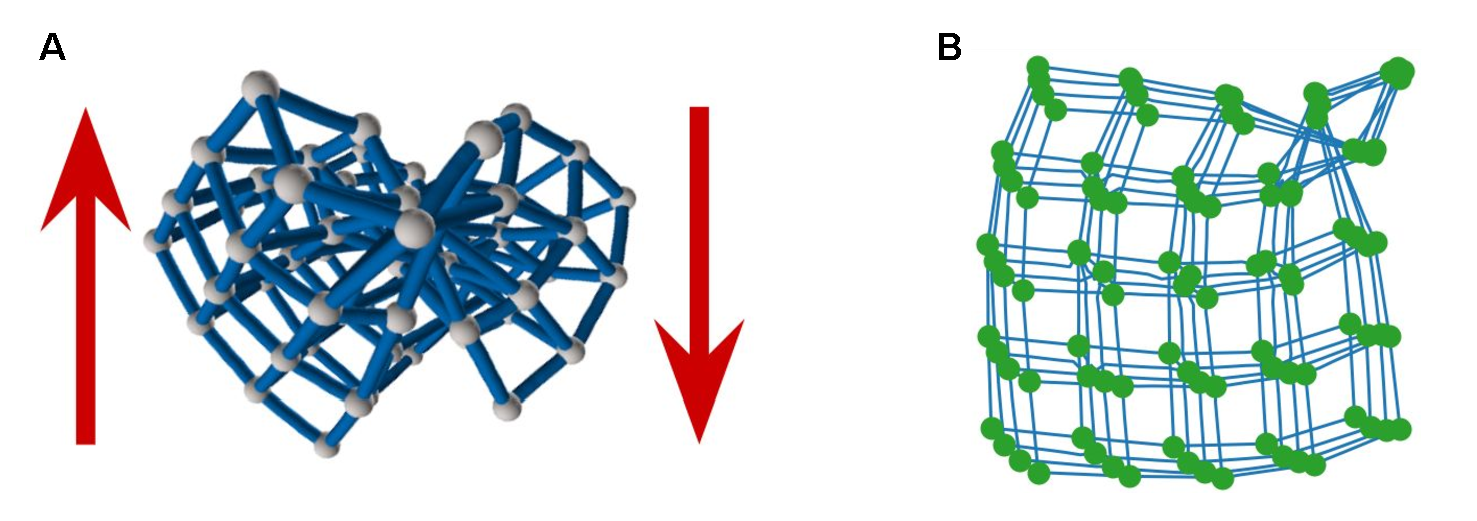
\includegraphics[width=.8\textwidth]{fig-09-19/3D-twist.pdf}
    \caption{{\bf Solitonic solutions:} A frequent outcome of laying out networks with discrete symmetries, such as 3D lattices due to reflection symmetry, is topological defects: the orientation of two ends of the lattice may be different (A, red arrows pointing to the fact that the orientation of the lattice along the y direction has switched from one end of the layout to the other), resulting in a twist in the middle of the layout. 
    (B) A clearer view of a twist in occurring in laying out a lattice. 
    Twists, like other solitonic solutions, are generally localized, increasing total link lengths only by a small amount. 
    As a result, these solitonic solutions have energies close to the global minimum.
    They are encountered frequently during simulated annealing because of their high degeneracy: the twist may occur anywhere in the lattice and its energy is related to its size. 
    }
    \label{fig:twist}
\end{figure}
The underlying reason is the same as regular solitons: there exist multiple global minima for $V$ which are related to each other via discrete symmetries, such as reflection in the $x$ direction. 
During the dynamics one side of the network may fall into one minimum configuration and the other side into the reflected configuration, resulting in a twist somewhere in the layout. 
These solitonic solutions are still low energy solutions. 
Even though they are not a global minimum, their energy is close to the global minimum and their number is more plentiful than the global minima because of the combinatorics. 
In fact, most layouts of the 3D lattice, including the ones used for Fig.2 turn out to have such twists, but in the log-scale, $\be{l}$ and curvature seem to be similar among them, suggesting that they belong to approximately degenerate energy states. 
We would be happy to discuss this further. 

\end{response}
\begin{response}{
15) Distribution of link length or curvature. Average link length is an important order parameter of phase transition. Instead of characterizing the order transition by a simple average, I suggest the authors to investigate the change of distribution of link length which will provide more details about how the transition happened.
}
This is an interesting proposal. 
We did look at distributions of forces in relation with the stress, but they differ across different topologies in the weak exclusion phase.
We couldn't find a reasonable universal measure that works across different topologies and at the same time found that the phase behavior had almost no dependence on the topology. 

\end{response}

~\newpage
~\newpage

\section{Add to Main Text}

\subsection{Computational Complexity}
If each link had $s$ segments, the  complexity of calculating the elastic forces will be $O(sL)$.
The brute-force complexity of node repulsion is $O(N^2)$ and link repulsion $O(s^2L^2)$.
Since for a connected network $L\geq N-1$ and $s>1$, the complexity is mostly due to link repulsion. 
We can reduce this complexity by realizing that we only need short-range link repulsion to avoid crossings, allowing us to partition the space into cells of size $ar_L$ with $10>a>2$ and calculate link crossings in these cells only, as the repulsive forces between links farther than $ar_L$ will be exponentially small.
To be specific, if the layout is broken into $k$ cubic cells, each cell contains $sL/k$ link segments, on average, and so the total number of pair interactions has complexity
$O(k\times s^2L^2/k^2 ) = O(s^2L^2/k)$ (SI 8.C). 
A fixed minimum number of cells, $k$, is desirable at early stages as links may be very densely packed and a cell of size $ar_L$ may contain too many segments, resulting in memory shortage from storing the $O(s^2L^2)$ interaction matrix in the worst case. 
When the system has opened up sufficiently, we can break the layout into cells of fixed size $ar_L$ and index which segments of which links cross each cell. 
The indexing is $O(sL)$ and is updated every few iterations, depending on the magnitude of forces.
% After the indexing, a cubic cell with side $ar_L$ contains $O(a^3)$ link segments in the worst case. 
We only need to calculate forces in cells that contain more than one link.
We also shift the cells randomly for each indexing event to remove biases at the cell walls. 


In the weak phase using cells speeds up calculations enormously, as the number of crossings is very few and so cells crossed by more than one link are very few. 
Thus the total complexity will be either $O(N^2)$ from brute-force node repulsion or $O(sL)$ from indexing link segments and elastic forces, depending on which one is bigger.
In the strong phase, the links are filling the space.
But, as links can shrink and stretch, both with no link self-repulsion (Eq.(1)) and the double-ellipsoid potential (SI C. Eq.(32)) the number of link segments within one cell can vary from $1$ segment per cell to $O(s)$ per cell in the worst case.
A cell of size $ar_L$ contains a maximum of $O(a^3)$ distinct links. 
Since links can shrink and stretch, the number of segments of each link that falls in each cell can vary. 
In the best case, a cell has $1$ segment per link, and in the worst case it contains all $s$ segments.
Thus, in the worst case one cell may have $O\pr{(sa^3)^2}$ pairs of interacting link segments. 
The number $n_a$ of spatial cells with links crossing through them can be estimated from the size of the layout. 
The cross-section of all the links when the layout has opened up is $R\sim L^{1/2} r_L$ and so dividing by the cell size $ar_L$, the number of cells becomes $n_a \sim O\pr{\pr{L^{1/2}/a}^3}$. 
Therefore, the worst case time complexity is 
\[n_a O\pr{(sa^3)^2} \sim  O\pr{{ s^2 a^3  L^{3/2} } } \]
In practice, because the number of pairs $s^2 a^6$ in a cell may become large, we randomly sample up to a maximum number of pairs $\sim \max (100, s^2 a^3)$ in each cell to calculate the repulsive forces and the elastic forces help move the rest of the link segments to the correct positions. 
This way, for large networks the complexity is mostly due to number of cells $O(L^{3/2}/a^3)$.
Our algorithm starts with a minimum number of cells $k$ and switches to cells of fixed size $ar_L$ once the network has opened up enough so that more than $k$ cells are occupied by more than one link. 

As in the weak phase link crossings are rare, most cells will contain a single link.
Thus, in the weak phase partitioning the space reduces the complexity of link repulsion so much that it may become less than the brute-force complexity of node repulsion, $O(N^2)$.
Therefore,  with partitioning the time complexity in the weak phase will be $\max\{O(N^2),O(sL)\}$, where $O(sL)$ is the complexity of partitioning the space (same as the elastic forces).
In practice, we do not partition the space in every iteration, rather every 50-100 steps. 


\subsection{Star-shaped Network}
Consider a star network: 
Node 1 is at the center and all other $N-1$ nodes are only connected to node 1. 
Note that we have a short-range repulsion between nodes, independent of their degree, resulting in exclusion radius $r_N$ around each node. 
The tightest way to pack the $N$ nodes of this star network is a 3D close-packing of spheres, which results in a radius $R_N\sim N^{1/3}r_N$.
We have $L=N-1$ links going out at all angles but also ending on the nodes.
Let us calculate the average link length to see how much volume these link with thickness $r_L$ occupy. 
The mean link radius is simply the average of node location in a sphere of radius $R_N$ 

\begin{align}
    R_L =  \frac{4\pi \int_0^{R_N} r^3dr }{\int_0^{R_N} 4\pi r^2 dr} = {3\over 4} R_N
    \label{eq:RL}
\end{align}
Therefore the total volume of links will be $V_L = \pi L r_L^2 R_L \approx 3\pi/4 L R_N r_L^2 $ when this volume is comparable to the total node volume $V_N = 4\pi/3 R_N^3$, the number of links pressing against each other becomes substantial and the phase transition occurs when
%
\[ {r_L\over r_N} = {3\over 4} N^{1/3}L^{-1/2}\]
%
Of course, the node layout that FDL will find won't be a perfect close-packing of spheres, but it will come close to it.
So, as expected, up to the numerical factor of $4/3$ our prediction for the phase transition is seems correct.


\subsection{Phase Transition}

In some cases the phase transition can be worked out explicitly. 
But first we need to understand the fundamental concept that leads to the transition. 
The behavior of the system changes when link volumes become so large that they push nodes apart. 
But links that are coming out of a point-like node will inevitably cross each other. 
For a node of degree $k$ and with link thickness $r_L$, the region where the crossings of links exiting this node is unavoidable can be found by considering the sphere with minimum radius $r_0$ around the node outside of which links do not overlap any more. 
On the surface of this sphere, all links are barely touching each other. 
So, the surface area of the sphere is covered by the total cross-section of the $k$ links. 
Naively, this will mean 
\[4\pi r_0^2 \approx k \pi r_L^2,\qquad \Rightarrow \qquad r_0 \approx {\sqrt{k}\over 2} r_L  \]
A slightly more accurate value for $k\gg 1$ can be found by realizing that the link cross-sections will arrange in a hexagonal lattice on the surface of the sphere and so the area occupied by each link is $2\sqrt{3} r_L^2$ instead of $\pi r_L^2$. 
Therefore
\[r_0 \approx  \sqrt{{ \sqrt{3} k \over 2\pi }} r_L \approx {\sqrt{k}\over 1.9 } r_L\]
which is not very different from the first approximation. 
$r_0$ is the minimum radius above which links will have enough space. 
Thus, if $r_0$ becomes comparable to the radius of the network based on close-packing the nodes, i.e. $R\sim N^{1/3} r_N$, the layout will transition to strong interaction phase. 
However, we need to consider the fact that not all nodes connected to the central node will be a distance larger than $r_0$ away from it. 
%In the star-shaped network the number of links is $L=N-1$ and 
Based on this, the minimum size of a region over which we look for crossings around a degree $k$ nodes must be larger than $r_0(k,r_L)$.


To find where the phase transition occurs, the first thing to check is how the volume of the links compares to the total volume of nodes. 
When they become comparable, the phase transition is inevitable. 
It may happen that density heterogeneity affects this, and we will work this case out as well.
But first, we consider the whole network.  
When link thickness is $r_L$, the $N$ links around the center hub can avoid each other only above a radius $r_0 = k^{1/2}_{\max} r_L /2 $ (SI 9). 
In the weak phase, the total radius of the layout (assuming the network is not much longer in one direction than other directions) $R_N \sim N^{1/3} r_N$. 
For a node of degree $k$ we have
\begin{align}
    r_0 & ={1\over 2}  k^{1/2} r_L, \quad R_L = c R_N \cr  
    V_L & = \pi k r_L^2 (R_L-r_0) + {4\pi\over 3} r_0^3 \cr 
    &= c\pi k R_N r_L^2 %+\pr{ {1\over 6}- {1\over 2} } \pi 
    - { \pi \over 3}k^{3/2} r_L^3  
    \label{eq:VL}
\end{align}
This expression for the link volume will be valid as long as the second term is smaller than the first, meaning
\[c N^{1/3} r_N >{\pi\over 3} k_{\max}^{1/2} r_L\]
so that the overlapping volume is not occupying the whole layout. 
This condition and the condition for the node volumes $V_N$ becoming comparable to the link volumes will determine the phase transition, depending on which one occurs at smaller $r_L/r_N$ ratio. 
Thus, for a node of degree $k$ we have
\begin{align}
    \alpha \pi N r_N^3 &\approx \pi r_L^3 \pr{c N^{1/3}L  {r_N \over r_L} 
    - { 1\over 3}N {k^{3/2}}}\cr 
    0 &= \alpha N \pr{{r_N\over r_L}}^3 -c N^{1/3} L  {r_N \over r_L} 
    + { 1\over 3}N {k^{3/2}} 
\end{align}
where $\alpha $ depends on how the spherical nodes are packed.
The volume occupied by $N$ close-packed spheres is not $4\pi N /3 r_N^3$, rather $4\sqrt{2} N r_N^3$ because spheres can occupy a maximum fraction of $3\pi/\sqrt{2}$ of the volume. 
So, in this case $\alpha = 4\sqrt{2}/\pi \approx 1.8$. 
In this case, it follows that 
\begin{align}
    0 &= \alpha \pr{{r_N\over r_L}}^3 -c N^{-2/3} L  {r_N \over r_L} 
    + { 1\over 3} {k^{3/2}} % 2^{5/2} 
    \label{eq:trans-full}
\end{align}

\subsubsection{Location and Width of the Transition Region}
From \eqref{eq:trans-full} we see that nodes with different degrees satisfy the condition at different $r_L/r_N$ ratios. 
In fact, the degree becomes irrelevant only in the limit of $N^{-2/3} L \to \infty$, which is satisfied for any connected graph when $N\to \infty$, because $L> N-1$ and so $N^{-2/3} L > N^{1/3}$.  
Thus, the asymptotic solution becomes
\begin{align}
    {r_L\over r_N} = \sqrt{{\alpha \over c}}%c^{-1/2} 2^{5/4} 
    N^{1/3}L^{-1/2} %\approx 2.75 \times N^{1/3}L^{-1/2}
\end{align}
In Erd\"os-Renyi random graphs, the value of $c$ can be calculated form the uniformity of the connectivity \eqref{eq:RL} to be $c=3/4$. This yields 
\[ \sqrt{{\alpha \over c}} \approx 0.87 \]
which is close to one and so we can neglect the prefactor entirely. 
Eq. \eqref{eq:trans-full} can also be solved exactly to get a more accurate estimate of the transition point. 
It has the form 
\begin{align}
    &\rho^3 - a \rho + b =0 & a&= {c\over \alpha} N^{-2/3} L ,
    \quad b={ k^{3/2}\over 3\alpha } 
    \label{eq:rhoab}
\end{align}
with $\rho \equiv r_N/r_L$.
Since the coefficient of $\rho^2$ is zero, the sum of its roots is zero, meaning that it has at least one positive and one negative root.
Also, since the product of the three roots is $-b$ and since here $b= \be{k^{3/2}}/3>0$, we definitely have two positive roots and one negative root. 
Finally, $-b = \rho_-(\rho_++\rho_0) +\rho_0\rho_+ <0$, with $(\rho_-,\rho_0,\rho_+)$ being the three roots in increasing order ($\rho_-<0$). 
This results in 
\[{1\over \rho_0} + {1\over \rho_+} > {1\over -\rho_-}\]
Since each node must have at least one link, the transition must occur at $r_N \geq r_L$, as multiple links may be fitted around a single node and before $r_L$ becomes as large as $r_N$, the links will collide. 
Thus, only the roots $\rho > 1$ are acceptable as a transition point. 

The root $\rho_+(k)$ can be written out explicitly
\begin{align}
    \rho_+(k) %& =\frac{8 \sqrt[3]{2} \cdot 3^{\frac{2}{3}} b + \sqrt[3]{12} x^{\frac{2}{3}} \left(1 + \sqrt{3} i\right)^{2}}{12 \sqrt[3]{x} \left(1 + \sqrt{3} i\right)}\cr 
    %&= \frac{8 \sqrt[3]{2} \cdot 3^{\frac{2}{3}} a + \sqrt[3]{12} A^{\frac{2}{3}}}{12 A^{\frac{1}{3}} }\cr
    %&= \frac{- \alpha^{\frac{2}{3}} + \sqrt{3} i \alpha^{\frac{2}{3}} + 24 b}{6 \sqrt[3]{\alpha} \left(1 + \sqrt{3} i\right)} \cr
    %&= \frac{ \alpha^{\frac{2}{3}} + 48 b}{12 \alpha^{\frac{1}{3}} } \cr
    &=\frac{A^{\frac{2}{3}} + 12 a}{6 \sqrt[3]{- A}}, &
    %A& = 2i^{{2\over 3}}\pr{9 b + \sqrt{3} \sqrt{- 4 a^{3} + 27 b^{2}}},\cr
    A& = 12 \pr{9 b + \sqrt{(9b)^{2}- 12 a^{3} }}
    \label{eq:trans-rc-full}
\end{align}
with $a,b$ same as \eqref{eq:rhoab}. 
The overall transition point or the network is then the average of the roots over the degree distribution
\begin{align}
    \ba{\rho}_c = \be{\rho_0(k)}
\end{align}
Similarly, the width of the transition region around $\rho_c$ can be estimated from the standard deviation $STD[\rho_0(k)]$, again, evaluated using the degree distribution.



\subsubsection{The width of the transition region}
Another factor that we wish to examine is how much the heterogeneity in the degrees affects the spread of the transition. 
The roots of \eqref{eq:trans-full} are a function of the 




\subsection{Random Graphs}
In Erd\"os-Renyi random graphs, the value of $c$ can be calculated form the uniformity of the connectivity \eqref{eq:RL} to be $c=3/4$. 


\outNim{
\subsubsection{General Comparison of Conditions}
We wish to find out which of the following two conditions occurs at smaller $r_L/r_N$ ratio: 1) total node volume becomes comparable to leading term of link volumes; 2) link exclusion volume becomes considerable. 
}

\subsubsection{Transition in Lattice and Random Geometric Graphs}
A key point about Lattices and random geometric graphs (RGG) is that their optimal layouts are approximately translationally invariant, meaning that they consist of similar unit cells repeating themselves. 
For instance, if a lattice or RGG consists of $M$ similar unit cells, each contains $N_c = N/M$ nodes and $L_c=L/M$ links. 
For each unit cell, the previously derived condition for a phase transition was 
\[{r_L\over r_N} \sim L_c^{-1/2} N_c^{1/3} = M^{-1/6} L^{-1/2} N^{1/3} \]
Since in a lattice the number of nodes in a unit cell is a fixed number $C$, the number of cells is actually a function of the number of nodes and this changes the scaling law to 
\[{r_L\over r_N} \sim \pr{{N\over C}}^{-1/6} L^{-1/2} N^{1/3} = C^{1/6} L^{-1/2} N^{1/6} \]
For a small network with $N\sim 100$ the extra factor of $N^{1/6}\sim 2$ may not be considerable in a log-log plot, but it can be measured in a large lattice or RGG. 

%The other term to consider is the negative link exclusion term in \eqref{eq:VL}. 
\begin{figure}
    \centering
    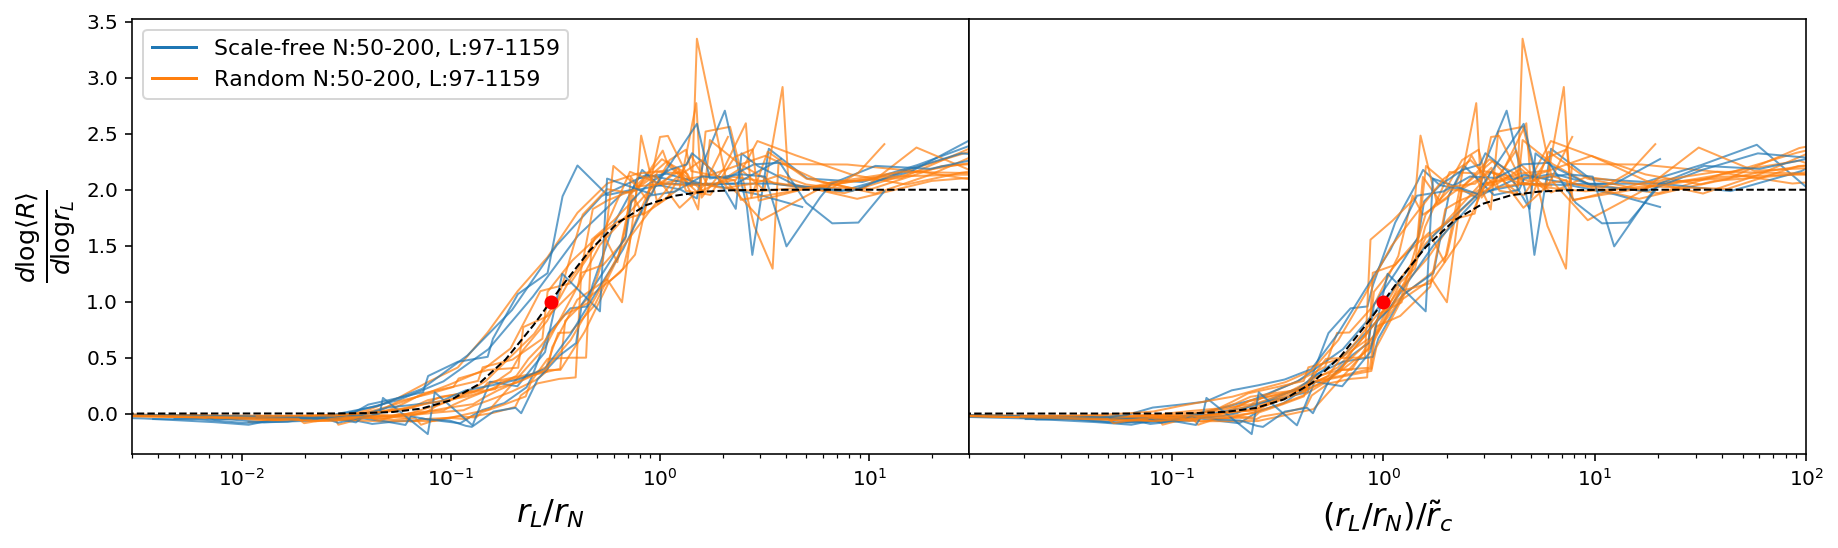
\includegraphics[width=\textwidth]{fig-09-19/phase-collapse-040918.png}
    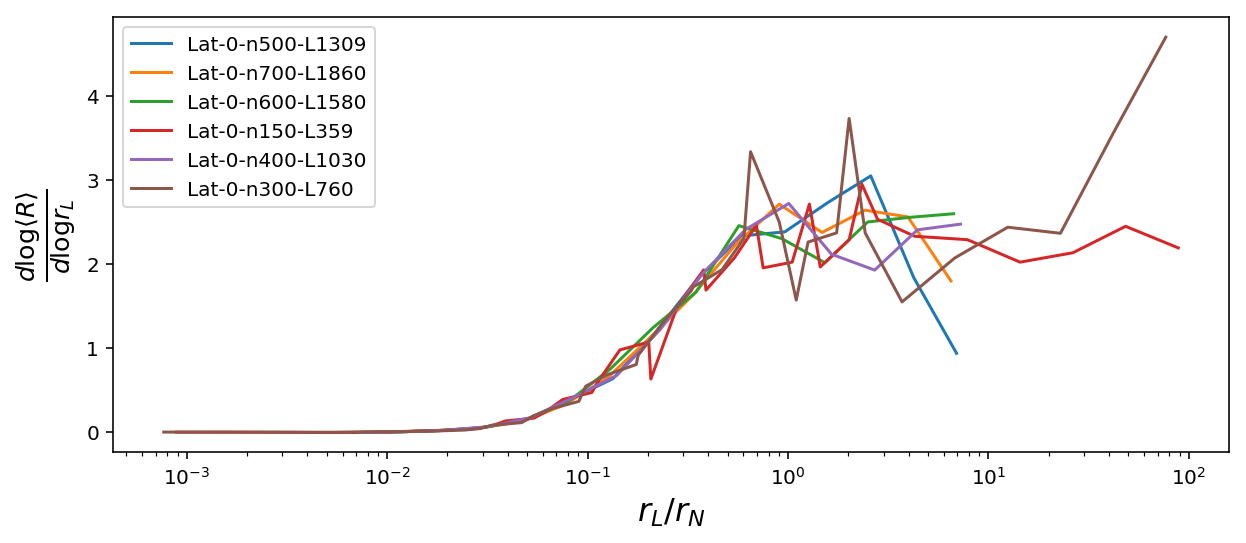
\includegraphics[width=.6\textwidth]{fig-09-19/phase-lat-040918.png}
    \caption{{\bf Phase transition vs Topology:} The quantity $\phi(r_L)\equiv d\log\be{R} /d\log r_L$ distinguishes well between the two phases  ($\be{R}$ being the average link length and keeping $r_N$ constant.)
    $\phi (r_L) $ is zero deep in the weak phase and it approaches $1$ deep in the strongly interacting phase. 
    While scale-free or random networks of various sizes network result in transitions occurring at different values of $r_L/r_N$ (Top, left), scaling by the predicted transition point $\tilde{r_c}=r^c_L/r_N$ collapses the curves well onto a single curve (Top, right).
    Lattice (Bottom) behave differently than random and scale-freee networks. 
    Lattice of all sizes have the same transition point, because once the unit cell has a phase transition the whole lattice udergoes a transition. 
    % If we start from the perfect lattice layout, the layout remains a lattice only gets slightly distorted at large $r_L$. 
    % The transition behavior in lattices is almost independent of the lattice size. 
    % 
    }
    \label{fig:phase-collapse}
\end{figure}


In lattice and RGG, all nodes have similar degrees $k = L/M$ and the average link length is the size of the unit cell so $R_L = c(N/M)^{1/3} r_N$. 
For close-packed nodes, $c \approx 3/4$. 
Thus, when the two terms in \eqref{eq:VL} become comparable we have 
\begin{align}
    {3\over 4} k R_L r_L^2 & \approx {1\over 3} k^{3/2} r_L^3 \cr 
    N^{1/3}M^{-1/3} r_N &\approx L^{1/2} M^{-1/2} r_L \cr
    {r_L \over r_N } &\approx M^{-1/6 } L^{-1/2} N^{1/3}
\end{align}
which is the same condition as the $V_L \sim V_N$ condition used to derive the transition point. 
In conclusion, for a lattice or RGG with close to optimal layout the phase transition should occcur at $r_c \sim N^{1/6} L^{1/2} $ instead of the previous estimate. 
If the layout is far from optimal with many defects and long links, the phase transition becomes closer to the random graph's $r_c \sim N^{1/3} L^{1/2}$. 



\subsubsection{Sclae-free network}


The coefficient $c$ depends on the distribution of nodes inside the layout which are linked to the node we are considering 

To get the total volume, we have to integrate this over the degree distribution $p(k) $. 
Since the first term is linear in $k$, we simply get the total number of links $L$. 
The second term, which is the correction due to overlapping part of the links, has the form $N \be{k^{3/2}}$. 
Thus, the second term can be regarded as one way that heterogeneity in degrees can affect the transition.
Nodes with higher degrees get a larger contribution from this term. 
In a uniform network, such as the ER random graph, $k\approx 2L/N$. 
The first term again yields the normal transition point {\color{red} calculate heterogeneous term explicitly!}

In the specific case of $\gamma =2 $ scale-free network $k_{max}=N$. 
Thus, for the central hub the volume occupied by these $N$ links is derived from their length and cross-section. 
If the hub node is placed at the center of the layout and if the nodes are occupying a volume with total radius $R_N\sim N^{1/3} r_N$, the average link length (SI 9) will be $R_L = 3/4 R_N$. 
% When the hub is not at the center, only the coefficient changes slightly
The total volume of these $N$ links is, thus, \begin{align}
    V_L %& = \pi k_{\max} r_L^2 (R_L-r_0) + {4\pi\over 3} r_0^3 \cr 
    &= \left[{3\pi \over 4} N^{1/3} {r_N \over r_L}  +\pr{ {1\over 8}- {\pi\over 2} } N^{1/2}\right] N r_L^3  
\end{align}
For a star-shaped network this would be the total link volume as $L=N-1$. 
Comparing this to the node volume $V_N = {4\pi \over 3} N r_N^3$, the first term yields a transition at
\[ {3\pi \over 4} N^{4/3} r_N  r_L^2 \approx  {4\pi \over 3} N r_N^3 \qquad \Rightarrow \qquad {r_L\over r_N} \approx {4\over 3} N^{-1/6} \approx {4\over 3} {N^{1/3}\over L^{1/2}} \]
compatible with our estimate. 
In general, it is straightforward to see what the power dependence on $N$ and $L$ should be. 
In the weak phase the volume of nodes goes with $r_N^3$, where as the volume of links goes as $R_L r_L^2$. 
The length of the link $R_L$ must come from the exclusion of nodes in the weak phase and thus must be proportional to $r_N$. 
The exact factor depends on the network topology. 
In another extreme, namely the lattice and random geometric graphs, the network approximately consists of repeating unit cells, each containing a fraction $N/M$ of nodes and $L/M$ of links. 
In this case, the expression for the transition point becomes 
\begin{align}
    {r_L\over r_N} \approx M^{-1/6} {N^{1/3}\over L^{1/2}}
\end{align}




% First, note that the estimation of the phase transition point is done up to numerical factors that will depend on the details of the network architecture.
% As you correctly point out, heterogeneity of the network will affect it, but not the way you describe it. 
%The underlying reason is that heterogeneous degree distribution does not guarantee that force-directed layouts (FDL) result in inhomogeneous spatial density of nodes. 
To discuss this, we first have to establish what we mean by ``near a hub'', i.e. we need to define the size of the neighborhood.
To capture statistical properties of the layout the size of the neighborhood needs to be at least large enough to capture all links coming out of any node. 
In particular, the neighborhood size should be able to capture all links of a hub, as these links are interacting with each other and a neighborhood that captures only part of this interaction cannot describe a potential phase transition correctly. 
As we explain in SI 7.A, a degree $k$ node in a an unweighted network will have overlapping links up to radius $r_0\sim \sqrt{k} r_L/2 $. 
Thus, the neighborhood size must have radius larger than $r_0$. 
To measure heterogeneity, we must fix the neighborhood size and measure the link density in different parts of the network. 
Therefore, we choose the neighborhood radius to be $r_0\sim \sqrt{k_{\max}} r_L  $, where $k_{\max}$ is the maximum degree in the network. 
When $r_L/r_N$ is small, neighborhoods of size $r_0$ mostly consists of the node itself and the links connected to it. 
Thus, for small $r_L/r_N$ density of links around hubs will be larger and there will in general be a strong correlation between degree and link density. 
For large $r_L/r_N$, however, this heterogeneity becomes weaker. 

\textbf{Figure \ref{fig:neigh}} shows the properties of the number of links in the vicinity of a node for a scale-free (Barabasi-Albert) network and a random (Erd\"os-Renyi) network, both with $N=100, L=197$. 
We are not running the full algorithm, rather we are using the Force-directed Layouts (FDL) with straight links to measure the density of links. 
As we see, the coefficient of variation $\sigma/\mu$ (\textbf{Figure \ref{fig:neigh}}, right) of the number of links in the neighborhood of different nodes is high below the transition point, meaning heterogeneity in density is considerable. 
However, this heterogeneity  drops quickly after the transition.  
The correlation between degree and number of links in the neighborhood of a node (\textbf{Figure \ref{fig:neigh}}, left) drops sharply in the scale-free  network near our predicted transition point. 
Thus, near the transition point, a reasonably large neighborhood of nodes shows only a weak correlation between link density and node degree in a scale-free network.
We may, therefore, ignore the heterogeneity in link density near or above the transition point. 
The reason for this sharp drop in heterogeneity is that low degree nodes are mostly connected to hubs and so a reasonably large neighborhood of any low-degree node contains a hub and the large number of links connected to it. Thus, the density of links becomes similar among hubs and low-degree nodes at such radii.  

The random network also exhibits a drop in this correlation around the transition point, but maintains a high correlation between the degree and the number of neighborhood links up to very high $r_L/r_N$. 
Of course, since the overall variation in degree in ER is small, this correlation does not signify a large heterogeneity in the density of links around nodes, and the density of the links is fairly homogeneous over space. 

\begin{figure}[ht]
    \centering
    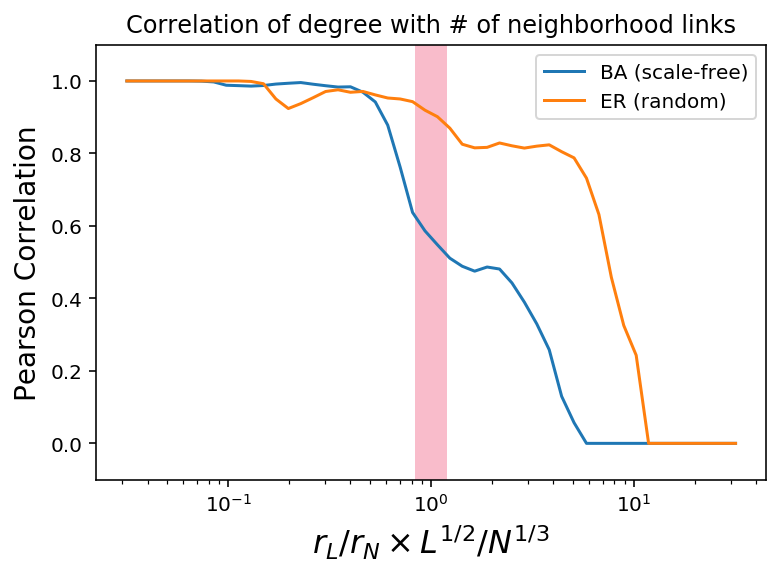
\includegraphics[width=.45\textwidth]{fig-09-19/corr-deg-neigh.png}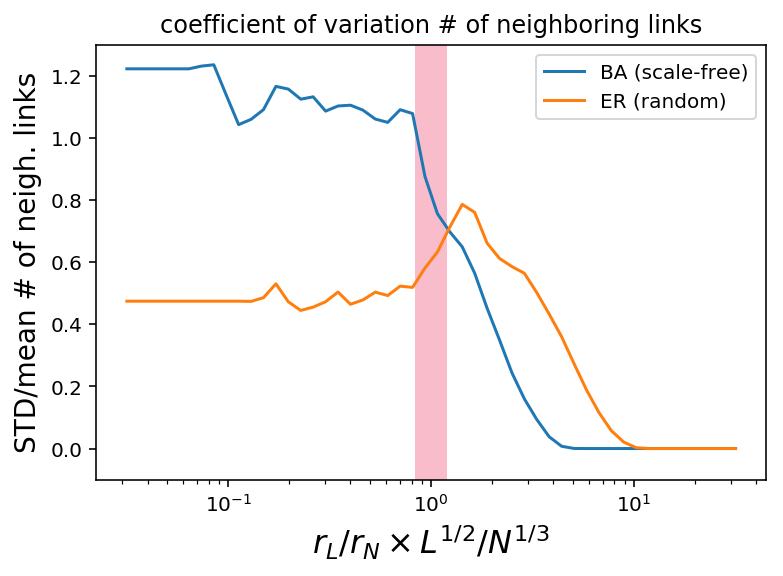
\includegraphics[width=.45\textwidth]{fig-09-19/coeff-var-neigh.png}
    \caption{{\bf Spatial heterogeneity of number of links in the neighborhood of nodes: }
    Correlation between degree and number of links in a neighborhood of radius $r_0\sim \sqrt{k_{\max}} r_L  $ of nodes in a scale-free and a random graph (Left) laid out using FDL (without links avoiding crossing) shows that the link density is correlated in with the degree. 
    But the correlation falls sharply above the transition point (red vertical band) in the scale-free network (blue curve).
    Thus, heterogeneity in link density becomes very weak near the phase transition and we can neglect it over a large region of the network.
    }
    \label{fig:neigh}
\end{figure}

Additionally, we would like to point out that Force-directed Layouts (FDL) are known to be equivalent to modularity clustering \cite{noack2009modularity}. 
Modularity $A_{ij}- k_ik_j/\pr{2\sum_l k_l}$, like degree assortativity, is a  second-order moment of the adjacency matrix and is not related to degree distribution. 
%It is well-known that Scale-free networks such as Barabasi-Albert have zero degree assortativity. 
Barabasi-Albert (BA) scale-free networks have vanishingly small modularity because they are ultra-small world and their degree assortativity is also zero. 
In particular, first order moments of the network, such as degree of nodes, does not result in the kind of heterogeneity in the density of links that would affect the transition point.
Having two modules with vastly different average degrees (e.g. two ER networks with different average degree connected to each other via a few links), however, does result in a  heterogeneity of link density which persists all the way until the neighborhood radius $r_0$ becomes comparable to the total layout radius. This kind of heterogeneity will change the behavior of the transition point.   
\outNim{
Consider a ball around a degree 1 node in a scale-free network. 
This node is most likely connected to a hub and the ball will therefore likely to contain the hub and other links connected to it.
This means that degree alone will not result in strong heterogeneity in the density of links. 
Also, note that, as we explain in SI 7.A, a degree $k$ node in a an unweighted network will have overlapping links up to radius $r_0\sim \sqrt{k} r_L/2 $ and to talk about the neighborhood of the node we have to talk about a region with radius larger than $r_0$.


Using FDL, inhomogeneous spatial node density only occurs in modular networks, not in scale-free networks. 
To see this, consider any low degree node in a scale-free network. 
We want to know if the links around it have lower density than around a high degree node. 
Take any link from a low-degree node.
In a scale-free network, the link is much more likely to be connected to a high degree node than a low degree node. 
Therefore the density of links around low degree nodes is practically the same as the density of links around high degree nodes, because neighbors of low degree nodes are mostly hubs.
There are no low density regions in a BA scale-free graph: the whole graph is mostly low-degree nodes connected to hubs. 
A random graph will clearly have a mostly uniform node distribution in space (except near boundaries of course), as all nodes look the same.
A highly modular network may undergo multiple transitions (this is the topic of our followup work). 
Of course, there can be modular graph  which are also approximately scale-free, in which case the referee's point would be valid.
More follows below. 
} 

Although, degree exponent alone, or being a lattice does not affect the transition, the referee raises a very important point which needs a careful answer.
A simple counter-example which shows Eq.(4) needs slight modification is the case of having two identical disconnected random graphs with $N$ nodes and $L$ links. 
According to Eq.(4), for each one of these the transition occurs at $\tilde{r}_c$. 
Obviously when the two netwrks are disconnected, the transition still occurs at $\tilde{r}_c$, but Eq.(4) predicts a different transition at $2^{-1/6}\tilde{r}_c$, which is clearly wrong. 
The reason for this is basically due to the point the referee is making, that the transition depends n local density. 
Following our answer to the previous question,  the real units that should be used in Eq.4 are the smallest ``modules'' in the network, similar to unit cells of a lattice.
In fact, Eq.(4) also fails if we consider lattices of different size.
%For a cubic lattice the transition occurs when $r_L\sim r_N $. 

{\color{red} To be continued...}

%Let us work on a specific example based on the referee's proposal.


\outNim{
The resolution is to use $N$ and $L$ of the 

What does matter is the size of the network and Eq.(4) is inaccurate unless we clarify the following. 
The main assumption of Eq.(4) is that the average length of links $R_L$ in any large region of the layout is the same. 
The accurate derivation of Eq.(4) comes from equating the total node volume $V_N \sim N r_N^3$ with the total link volume $V_L \sim R_L r_L^2$. 
Eq.(4) assumes that $R_L = c r_N $ is comparable to the layout radius. 
{\color{red}But this clearly fails in a 3D lattice and  geometric graphs. Talk about smallest unit cell that is repeated in these networks. The unit cell is what determines $N$ and $L$ to be used in Eq.(4). This will also solve the scaling issue.  }  
Eq.(4) predicts a transition when 
\[ \tilde{r}_c = {r_L\over r_N} = N^{1/3}L^{-1/2}\]
This would mean that if we double the number of nodes and links the transition would occur at $2^{-1/6} \tilde{r}_c$. 
However, in the weak phase a perfect cubic 3D lattice has $R_L=2r_N$ everywhere, regardless of the size of the lattice.
In a random graph, $R_L$ should grow uniformly with the layout radius, which itself grows with $N^{1/3}$ so $\tilde{r}_c$ does change. 


For the case of a lattice, in the perfect layout (i.e. lattice with no defect) the average link length is $R_L = 2r_N$. 
The number of links per node is $1$, so $L=N$. 
But this time, the average volume per each node is a cube of volume $r_N^3$ and the average volume excluded by each link not a cylinder, but a cuboid of volume $R_Lr_L^2$. 
Therefore, the link and node volumes become comparable when the thickness $r_L = r_N$ which is compatible with 
\[{r_L\over r_N} = \]
}



%A network can be a very heterogeneous object. 
To examine its physical properties we require a fixed scale over at which we could examine all parts of the system. 
$r_0$ sets a minimum scale for each node and at scales smaller than $r_0$ we will not capture the full properties of the links connected to the node, rather pieces of it.
Therefore to describe the phase properties of the network we must choose a scale larger than the largest $r_0$ such as 
\begin{equation}
    r_1 = 2r_0\pr{k_{\max},r_L} = \sqrt{k_{\max}} r_L 
\end{equation}
In the case of a power law degree distribution we have $p(k) = (\gamma-1) k^{\gamma-1}_{\min{}} k^{-\gamma}$ and $k_{\max} = N^{1/(\gamma-1)}$.
Setting $k_{\min} = 1$, for $\gamma >2$ the total number of links can be calculated as 
\begin{align}
    L &= {1\over 2} \sum_{i=1}^N k_i  = {N\over 2} \int_{1 }^{k_{\max}} p(k) k dk\cr
    &= {N(\gamma -1)\over 2 (2-\gamma )} \pr{N^{{2-\gamma\over \gamma -1}}-1} 
\end{align}
which for $\gamma =3 $ yields a tree with $L= N-1$. 
$\gamma =2$ is a special case where $k_{\max} = N$ and \begin{align}
    L = {N\over 2} \int_1^N k^{-1} dk = {N\over 2} \ln N
\end{align}

{\color{red} Even though $k_{\max}= N$, not all links come from the hub node. 
Having $N\ln N$ links means that other nodes also have a considerable number of links. 
In particular, one network that has this number of links wold be a hierarchical network in which a node at every level is connected to all nodes in the levels below it. 
The number of nodes from one level to the next increases by a factor $\alpha = N^{1/l}$ where $l$ is the number of levels. 

%with $\log N$ levels
}
%Since $k_{\max}= N$ at $\gamma=2$ we have a star-shaped network with all nodes essentially connected to a single node. 

Let us examine the scale-free case with mentioned by the referee with $\gamma=2$. 
In this case, there exists one hub with degree $k_{\max} = N$ (other hubs exist too, but with a fraction of this degree; see SI 9). 


{\color{red} Work out extreme cases
\begin{enumerate}
    \item $\gamma=2$ star-shaped
    \item scale-free
    \item Lattice and random geometric
    \item discuss two loosely connected modules.
    
\end{enumerate}


}


\bibliographystyle{plain}
\bibliography{mybib}
\end{document}